O texto \cite{dastaniframework} apresenta um modelo com a finalidade de descrever agentes normativos com a capacidade de cometer uma certa violação. O modelo define sanções para as violações. O estudo estrutura o modelo como uma linguagem de programação (usando a notação EBNF) onde os problemas de sistemas multiagentes são tratados como programas escritos neste linguagem \cite{dastaniframework}. Assim sendo, um programa de sistemas multi-agentes é descrito como sendo; 

\begin{figure}[H]
  \centering
  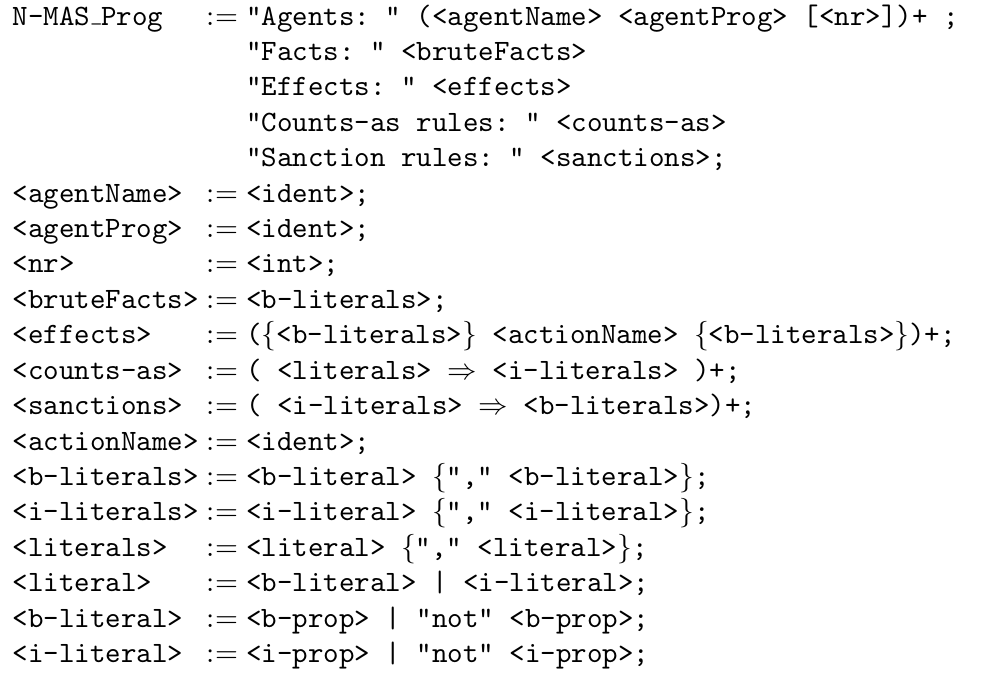
\includegraphics[width=0.8\linewidth]{figure/masprogram.png} 
  \caption{Linguagem para descrever um programa de multiagentes normativos com a possibilidade de violações e sanções na notação EBNF segundo o texto \cite{dastaniframework}. Nesta notação, $<ident>$ é usado para denotar uma \textit{string} e $<int>$ inteiros. Os termos $<b-prop>$ e $<i-prop>$ são usados para designar dois tipos de conjuntos de proposições que são disjuntos entre sí}
  \label{descreveprograma}
\end{figure}
